\documentclass[10pt,a4paper,journal,cspaper,compsoc]{IEEEtran}

% Some very useful LaTeX packages include:
% (uncomment the ones you want to load)

% *** CITATION PACKAGES ***
%
\ifCLASSOPTIONcompsoc
  % IEEE Computer Society needs nocompress option
  % requires cite.sty v4.0 or later (November 2003)
  \usepackage[nocompress]{cite}
\else
  % normal IEEE
  \usepackage{cite}
\fi
% cite.sty was written by Donald Arseneau
% V1.6 and later of IEEEtran pre-defines the format of the cite.sty package
% \cite{} output to follow that of IEEE. Loading the cite package will
% result in citation numbers being automatically sorted and properly
% "compressed/ranged". e.g., [1], [9], [2], [7], [5], [6] without using
% cite.sty will become [1], [2], [5]--[7], [9] using cite.sty. cite.sty's
% \cite will automatically add leading space, if needed. Use cite.sty's
% noadjust option (cite.sty V3.8 and later) if you want to turn this off.
% cite.sty is already installed on most LaTeX systems. Be sure and use
% version 4.0 (2003-05-27) and later if using hyperref.sty. cite.sty does
% not currently provide for hyperlinked citations.
% The latest version can be obtained at:
% http://www.ctan.org/tex-archive/macros/latex/contrib/cite/
% The documentation is contained in the cite.sty file itself.
%
% Note that some packages require special options to format as the Computer
% Society requires. In particular, Computer Society  papers do not use
% compressed citation ranges as is done in typical IEEE papers
% (e.g., [1]-[4]). Instead, they list every citation separately in order
% (e.g., [1], [2], [3], [4]). To get the latter we need to load the cite
% package with the nocompress option which is supported by cite.sty v4.0
% and later. Note also the use of a CLASSOPTION conditional provided by
% IEEEtran.cls V1.7 and later.


% *** GRAPHICS RELATED PACKAGES ***
%
  \usepackage[pdftex]{graphicx}
  \graphicspath{{../Figures/}}
  \DeclareGraphicsExtensions{.pdf,.png}
  \usepackage{color}

% *** MATH PACKAGES ***
%
\usepackage[cmex10]{amsmath}
% A popular package from the American Mathematical Society that provides
% many useful and powerful commands for dealing with mathematics. If using
% it, be sure to load this package with the cmex10 option to ensure that
% only type 1 fonts will utilized at all point sizes. Without this option,
% it is possible that some math symbols, particularly those within
% footnotes, will be rendered in bitmap form which will result in a
% document that can not be IEEE Xplore compliant!
%
% Also, note that the amsmath package sets \interdisplaylinepenalty to 10000
% thus preventing page breaks from occurring within multiline equations. Use:
%\interdisplaylinepenalty=2500
% after loading amsmath to restore such page breaks as IEEEtran.cls normally
% does. amsmath.sty is already installed on most LaTeX systems. The latest
% version and documentation can be obtained at:
% http://www.ctan.org/tex-archive/macros/latex/required/amslatex/math/

%\usepackage{amssymb}%............................ AMS Symbol fonts



% *** SPECIALIZED LIST PACKAGES ***
%
%\usepackage{algorithmic}
% algorithmic.sty was written by Peter Williams and Rogerio Brito.
% This package provides an algorithmic environment for describing algorithms.
% You can use the algorithmic environment in-text or within a figure
% environment to provide for a floating algorithm. Do NOT use the algorithm
% floating environment provided by algorithm.sty (by the same authors) or
% algorithm2e.sty (by Christophe Fiorio) as IEEE does not use dedicated
% algorithm float types and packages that provide these will not provide
% correct IEEE style captions. The latest version and documentation of
% algorithmic.sty can be obtained at:
% http://www.ctan.org/tex-archive/macros/latex/contrib/algorithms/
% There is also a support site at:
% http://algorithms.berlios.de/index.html
% Also of interest may be the (relatively newer and more customizable)
% algorithmicx.sty package by Szasz Janos:
% http://www.ctan.org/tex-archive/macros/latex/contrib/algorithmicx/

% *** ALIGNMENT PACKAGES ***
%
\usepackage{array}
% Frank Mittelbach's and David Carlisle's array.sty patches and improves
% the standard LaTeX2e array and tabular environments to provide better
% appearance and additional user controls. As the default LaTeX2e table
% generation code is lacking to the point of almost being broken with
% respect to the quality of the end results, all users are strongly
% advised to use an enhanced (at the very least that provided by array.sty)
% set of table tools. array.sty is already installed on most systems. The
% latest version and documentation can be obtained at:
% http://www.ctan.org/tex-archive/macros/latex/required/tools/


\usepackage{mdwmath}
\usepackage{mdwtab}
% Also highly recommended is Mark Wooding's extremely powerful MDW tools,
% especially mdwmath.sty and mdwtab.sty which are used to format equations
% and tables, respectively. The MDWtools set is already installed on most
% LaTeX systems. The lastest version and documentation is available at:
% http://www.ctan.org/tex-archive/macros/latex/contrib/mdwtools/

% IEEEtran contains the IEEEeqnarray family of commands that can be used to
% generate multiline equations as well as matrices, tables, etc., of high
% quality.

% *** SUBFIGURE PACKAGES ***
\ifCLASSOPTIONcompsoc
  \usepackage[caption=false,font=normalsize,labelfont=sf,textfont=sf]{subfig}
\else
  \usepackage[caption=false,font=footnotesize]{subfig}
\fi

%Setting captions to centered (Not IEEE journal standard)
%\makeatletter
%\long\def\@makecaption#1#2{\ifx\@captype\@IEEEtablestring%
%\footnotesize\begin{center}{\normalfont\footnotesize #1}\\
%{\normalfont\footnotesize\scshape #2}\end{center}%
%\@IEEEtablecaptionsepspace
%\else
%\@IEEEfigurecaptionsepspace
%\setbox\@tempboxa\hbox{\normalfont\footnotesize {#1.}~~ #2}%
%\ifdim \wd\@tempboxa >\hsize%
%\setbox\@tempboxa\hbox{\normalfont\footnotesize {#1.}~~ }%
%\parbox[t]{\hsize}{\normalfont\footnotesize \noindent\unhbox\@tempboxa#2}%
%\else
%\hbox to\hsize{\normalfont\footnotesize\hfil\box\@tempboxa\hfil}\fi\fi}
%\makeatother


% *** FLOAT PACKAGES ***
%
\usepackage{fixltx2e}
% fixltx2e, the successor to the earlier fix2col.sty, was written by
% Frank Mittelbach and David Carlisle. This package corrects a few problems
% in the LaTeX2e kernel, the most notable of which is that in current
% LaTeX2e releases, the ordering of single and double column floats is not
% guaranteed to be preserved. Thus, an unpatched LaTeX2e can allow a
% single column figure to be placed prior to an earlier double column
% figure. The latest version and documentation can be found at:
% http://www.ctan.org/tex-archive/macros/latex/base/

% *** PDF, URL AND HYPERLINK PACKAGES ***
%
\usepackage{url}

\usepackage{sistyle}
    \SIstyle{S-Africa}
    \SIunitspace{{\cdot}}
    \SIunitdot{{\cdot}}

% generate nice bookmarks and hyperrefs when exporting to pdf and dvi (screen version):
\usepackage[a4paper,plainpages=false,colorlinks,linktocpage,bookmarks=true,bookmarksopen=false]{hyperref}
% use this for printing only (no color, print version):
%\usepackage[a4paper,plainpages=false,colorlinks=false,linktocpage,bookmarks=true,bookmarksopen=false]{hyperref}

% correct bad hyphenation here
\hyphenation{op-tical net-works semi-conduc-tor}

%Add elegant support for Big-O notation
\providecommand{\OO}[1]{\operatorname{O}\left(#1\right)}

\begin{document}

%
% paper title
\title{A Hybrid Multi-Tiered State Persistency Model for Peer-to-Peer Massively Multiplayer Online Games}

\author{John~S.~Gilmore~and~Herman~A.~Engelbrecht% <-this % stops a space
\IEEEcompsocitemizethanks{\IEEEcompsocthanksitem J.S. Gilmore and H.A. Engelbrecht are with the MIH Media Laboratory at the Department of Electrical
and Electronic Engineering, Stellenbosch University, Stellenbosch, South Africa.\protect\\
% note need leading \protect in front of \\ to get a newline within \thanks as
% \\ is fragile and will error, could use \hfil\break instead.
E-mail: jgilmore@ml.sun.ac.za and hebrecht@sun.ac.za}% <-this % stops a space
\thanks{}}

\author{John~S.~Gilmore~and~Herman~A.~Engelbrecht% <-this % stops a space
\IEEEcompsocitemizethanks{\IEEEcompsocthanksitem J.S Gilmore is a PhD student at the MIH Media Laboratory at the Department of Electrical
and Electronic Engineering, Stellenbosch University, Stellenbosch, South Africa.\protect\\
% note need leading \protect in front of \\ to get a newline within \thanks as
% \\ is fragile and will error, could use \hfil\break instead.
E-mail: jgilmore@ml.sun.ac.za
\IEEEcompsocthanksitem H.A. Engelbrecht is the research manager at the MIH Media Laboratory.\protect\\
E-mail: hebrecht@sun.ac.za}% <-this % stops a space
\thanks{}}

% The paper headers
%\markboth{Draft Submission to the Journal of Parallel and Distributed Systems, July~2010}%
%{Draft Submission to the Journal of Parallel and Distributed Systems, July~2010}
% The only time the second header will appear is for the odd numbered pages
% after the title page when using the twoside option.

% The publisher's ID mark at the bottom of the page is less important with
% Computer Society journal papers as those publications place the marks
% outside of the main text columns and, therefore, unlike regular IEEE
% journals, the available text space is not reduced by their presence.
% If you want to put a publisher's ID mark on the page you can do it like
% this:
%\IEEEpubid{0000--0000/00\$00.00~\copyright~2007 IEEE}
% or like this to get the Computer Society new two part style.
%\IEEEpubid{\makebox[\columnwidth]{\hfill 0000--0000/00/\$00.00~\copyright~2007 IEEE}%
%\hspace{\columnsep}\makebox[\columnwidth]{Published by the IEEE Computer Society\hfill}}
% Remember, if you use this you must call \IEEEpubidadjcol in the second
% column for its text to clear the IEEEpubid mark (Computer Society jorunal
% papers don't need this extra clearance.)

% for Computer Society papers, we must declare the abstract and index terms
% PRIOR to the title within the \IEEEcompsoctitleabstractindextext IEEEtran
% command as these need to go into the title area created by \maketitle.
\IEEEcompsoctitleabstractindextext{%
\begin{abstract}
%\boldmath
The abstract goes here

\end{abstract}}
% IEEEtran.cls defaults to using nonbold math in the Abstract.
% This preserves the distinction between vectors and scalars. However,
% if the journal you are submitting to favors bold math in the abstract,
% then you can use LaTeX's standard command \boldmath at the very start
% of the abstract to achieve this. Many IEEE journals frown on math
% in the abstract anyway. In particular, the Computer Society does
% not want either math or citations to appear in the abstract.

% Note that keywords are not normally used for peer review papers.
%\begin{IEEEkeywords}
%A.1.0 [\textbf{Introductory and Survey}], C.2.d [\textbf{Distributed Systems}]: Distributed applications, J.8.g [\textbf{Internet Applications}]:
%Games
%\end{IEEEkeywords}
% make the title area
\maketitle

% To allow for easy dual compilation without having to reenter the
% abstract/keywords data, the \IEEEcompsoctitleabstractindextext text will
% not be used in maketitle, but will appear (i.e., to be "transported")
% here as \IEEEdisplaynotcompsoctitleabstractindextext when compsoc mode
% is not selected <OR> if conference mode is selected - because compsoc
% conference papers position the abstract like regular (non-compsoc)
% papers do!
\IEEEdisplaynotcompsoctitleabstractindextext
% \IEEEdisplaynotcompsoctitleabstractindextext has no effect when using
% compsoc under a non-conference mode.

% For peer review papers, you can put extra information on the cover
% page as needed:
% \ifCLASSOPTIONpeerreview
% \begin{center} \bfseries EDICS Category: 3-BBND \end{center}
% \fi
%
% For peerreview papers, this IEEEtran command inserts a page break and
% creates the second title. It will be ignored for other modes.
\IEEEpeerreviewmaketitle

\IEEEdisplaynotcompsoctitleabstractindextext

%\section{Introduction}
% Computer Society journal papers do something a tad strange with the very
% first section heading (almost always called "Introduction"). They place it
% ABOVE the main text! IEEEtran.cls currently does not do this for you.
% However, You can achieve this effect by making LaTeX jump through some
% hoops via something like:
%
\ifCLASSOPTIONcompsoc
  \noindent\raisebox{2\baselineskip}[0pt][0pt]%
  {\parbox{\columnwidth}{\section{Introduction}\label{sec:introduction}%
  \global\everypar=\everypar}}%
  \vspace{-1\baselineskip}\vspace{-\parskip}\par
\else
\section{Introduction}\label{sec:introduction}\par
\fi
%
% Admittedly, this is a hack and may well be fragile, but seems to do the
% trick for me. Note the need to keep any \label that may be used right
% after \section in the above as the hack puts \section within a raised box.

% The very first letter is a 2 line initial drop letter followed
% by the rest of the first word in caps (small caps for compsoc).
%
% form to use if the first word consists of a single letter:
% \IEEEPARstart{A}{demo} file is ....
%
% form to use if you need the single drop letter followed by
% normal text (unknown if ever used by IEEE):
% \IEEEPARstart{A}{}demo file is ....
%
% Some journals put the first two words in caps:
% \IEEEPARstart{T}{his demo} file is ....
%

%P2P MMOG Background
\IEEEPARstart{P}{eer-to-Peer (P2P)} Massively Multiplayer Online Games (MMOGs) have received significant attention from the research community, since
the first publication on the subject by Knutssonn et al. in 2004 \cite{knutsson_p2p_first}. P2P MMOGs promise to solve many issues prevalent in
today's Client/Server (C/S) based MMOGs. Some key issues have to be solved before P2P MMOGs can be implemented commercially. Over the past few years,
researchers have been addressing these challenges.

%Key challenges and focus
A recent article has identified six key challenges of P2P systems: Interest Management, Game Event Dissemination, Non-player Character (NPC) Host
Allocation, Game State Persistency, Cheating Mitigation and Incentive Mechanisms \cite{Fan_deisgn_issues_p2p}. Most of the challenges mentioned have
received significant attention from the research community, except for state persistency.

The focus of this paper is exclusively on one of the key challenges present in P2P MMOGs, namely: state persistency. The implementation of state
persistency in P2P MMOGs allows for the storage of game data. The fact that game data must now be distributed amongst various peers in the network
creates challenges not usually present in classic C/S MMOGs.

%Current techniques not perfect
This paper shows that none of the approaches to state persistency has thus far been sufficient to meet the storage requirements of MMOGs of today.
All storage models are evaluated according to the identified requirements of scalability, fairness, reliability, responsiveness and security.

%Propose multi-tiered model
Because current state persistency models do not address all the requirements of modern MMOGs, a novel hybrid multi-tiered state persistency model is
proposed that is based on grouping players in some logical way and allowing for responsive interaction between players in the same group, with lower
levels of responsiveness between groups.

%Implementation
The proposed multi-tiered model is currently being implemented in Oversim, a peer-to-peer simulation environment based in Omnet++. The model allows
for the measurement of the requirements of scalability, fairness, reliability and responsiveness. Furthermore, it allows for the comparison of the
current model with other state persistency models. Multiple P2P routing overlays have already been implemented in Oversim, which makes it possible
for the substitution of different overlays and comparing the results.

%Promising preliminary results
Initial results seem promising, with the implemented model functioning as expected. The system shows to be very responsive when storing data within a
group and as responsive as storing data in an overlay when storing data between groups.

%Summary
Section \ref{current_models} groups storage models found in the literature and describes the advantages and disadvantages of each group. The section
concludes with a comparison of the different storage models and comments on their applicability to P2P MMOGs.
%
Section \ref{proposed_model} introduces our proposed state persistency model and describes the different assumptions on which it is based.
%
Section \ref{implementation} describes the implementation details of the proposed model.
%
Section \ref{results} presents some preliminary results.
%
Section \ref{conclusion} concludes with a summary of the paper and a discussion on possible future work.

\section{Current state persistency models}
\label{current_models}

%Overview of four approaches
Four approaches have been identified by which state persistency is achieved in P2P MMOGs. These are: \emph{super peer storage}, \emph{overlay
storage}, \emph{distance-based storage} and \emph{hybrid storage}. Requirements have also been identified by which storage systems should be
measured. These are: scalability, fairness, reliability, responsiveness and security.

To clarify what type of objects are stored in these types, only the root objects, also called the authoritive objects, are considered for storage. It
is still assumed that replica objects that are used by players to render the world are locally stored and that these objects derive their states from
the respective root objects.

\begin{table*}[htbp]
\centering
\begin{tabular}{|r|c|c|c|c|l|}
\hline
Storage type & Reliability & Responsiveness & Security & Fairness & Examples\\
\hline
Super Peer & Medium & High & Low & Low & \cite{knutsson_p2p_first}\\
Overlay & High & Low & Medium & High & \cite{Douglas05enablingmassively}, \cite{using_freenet_storage},
\cite{Fan_phd}, \cite{past_storage_focus}\\
Hybrid & High & High & Medium & Low & \cite{zoned_federation}, \cite{hybrid_storage1}\\
Distance-based & Medium & High & Low & Medium & \cite{Buyukkaya_voronoi_state_management}, \cite{Hu_voronoi_IM},
\cite{colyseus_distance_based}, \cite{solipsis}\\
\hline
\end{tabular}
\caption{Differences between storage mechanisms} \label{tab_storage}
\end{table*}
%
Table \ref{tab_storage} presents a characterisation of current storage systems according to the characteristics defined. Table \ref{tab_storage} also
provides some references that act as examples of the different storage types mentioned. These example architectures will be discussed briefly in the
sections to follow.

\subsection{Super peer storage}

%Super peer storage - description
Super peer storage relies on the super peer storing all information that is in its domain. A domain is usually created by segmenting the world into
regions and super peers act as regional servers to all peers in their region. Each super peer handles state persistency for its region, hosting NPCs,
objects and persistent player data.

This storage method is much like a Client/Server setup, with the super peer acting as the server for the virtual geographic region assigned to it.

%Advantages/Disadvantages

\subsection{Overlay storage}

%Description

%Advantages/Disadvantages

\subsection{Hybrid storage}

%Description

%Advantages/Disadvantages

\subsection{Distance-based storage}

%Description

%Advantages/Disadvantages

\subsection{Summary and comparison}

\section{Proposed state persistency model}
\label{proposed_model}

\subsection{Multi-tiered}

\subsection{Grouping}

\subsection{Distance-based}

\section{Implementation}
\label{implementation}

\subsection{Oversim architecture}

\begin{figure*}[htbp]
 \centering
 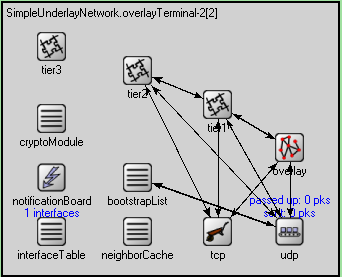
\includegraphics[width=\columnwidth]{Oversim_arch}
 \caption{Oversim architecture set up to use two tiers}
 \label{fig_oversim_arch}
\end{figure*}

\subsection{Components}

\begin{figure*}[htbp]
\centering \subfloat[Peer)]{\label{fig_p2p_cm}
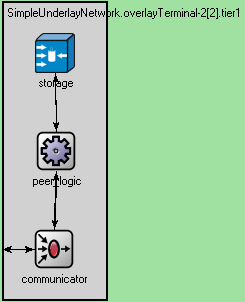
\includegraphics[width=0.815\columnwidth]{tier1_peer}}
 \subfloat[Super Peer]{\label{fig_cs_cm}
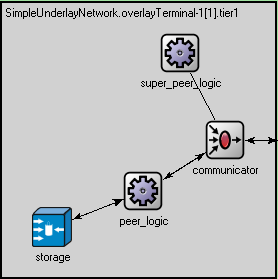
\includegraphics[width=\columnwidth]{tier1_super_peer}}
\caption{Tier 1 modules}
\end{figure*}

\section{Preliminary results}
\label{results}

\section{Conclusion}
\label{conclusion}

\subsection{Summary}

\subsection{Future work}


%\newpage
% use section* for acknowledgement
\ifCLASSOPTIONcompsoc
  % The Computer Society usually uses the plural form
  \section*{Acknowledgments}
\else
  % regular IEEE prefers the singular form
  \section*{Acknowledgment}
\fi

The financial assistance of MIH and the National Research Foundation (NRF) towards this research is hereby acknowledged. Opinions expressed and
conclusions arrived at, are those of the author and are not necessarily to be attributed to MIH or the NRF.

%\newpage
%\IEEEtriggeratref{43} %Balance the bibliography
\bibliographystyle{IEEEtran}
\bibliography{../BibTeX/P2P_MMOG}

% that's all folks
\end{document}
